\documentclass[journal,12pt,twocolumn]{IEEEtran}
\usepackage{graphicx}
\graphicspath{{./figs/}}{}
\usepackage{amsmath,amssymb,amsfonts,amsthm}
\newcommand{\myvec}[1]{\ensuremath{\begin{pmatrix}#1\end{pmatrix}}}
\providecommand{\norm}[1]{\lVert#1\rVert}
\usepackage{listings}
\usepackage{watermark}
\usepackage{titlesec}
\usepackage{caption}
\let\vec\mathbf
\lstset{
frame=single, 
breaklines=true,
columns=fullflexible
}
\thiswatermark{\centering \put(0,-105.0){
\includegraphics[scale=0.15]{/sdcard/IITH/vector/vector-1/figs/logo2.png}} }
\title{\mytitle}
\title{
Assignment - Vector
}
\author{Surajit Sarkar}
\begin{document}
\maketitle
\tableofcontents
\bigskip
\section{\textbf{Problem}}
Find the distance between the point(0,0) and (36,15).Can you now find the distance between the two towns A and B discussed in Section 7.2
\section{\textbf{Solution}}
The distance betwen the points A and B is given
\begin{align}
\vec{A}&=\myvec{0 & 0}\\ 
\Vec{B}&=\myvec{36 & 15} \\
&\norm{\vec{A}-\vec{B}}\\
\end{align}
where
\begin{align}
\vec{A}-\vec{B}&=\myvec{-36\\-15} \\
\vec{d}&=\sqrt{\myvec{\vec{A}-\vec{B}}^T\myvec{\vec{A}-\vec{B}}}\\
&=\sqrt{\myvec{-36\\-15}{\myvec{-36-15}}}\\
&=\sqrt{1296+225} &\\
&=\sqrt{1521} &\\
&=39
\end{align}
\section{\textbf{Code Link}}
\begin{lstlisting}
https://github.com/sssurajit/fwc/blob/main/vector/vector-1/codes/vector.py
\end{lstlisting}
Execute the code by using the command\\
\textbf{python3 vector.py}\\
\section{\textbf{Figure}}
\begin{figure}[!ht]
    \centering
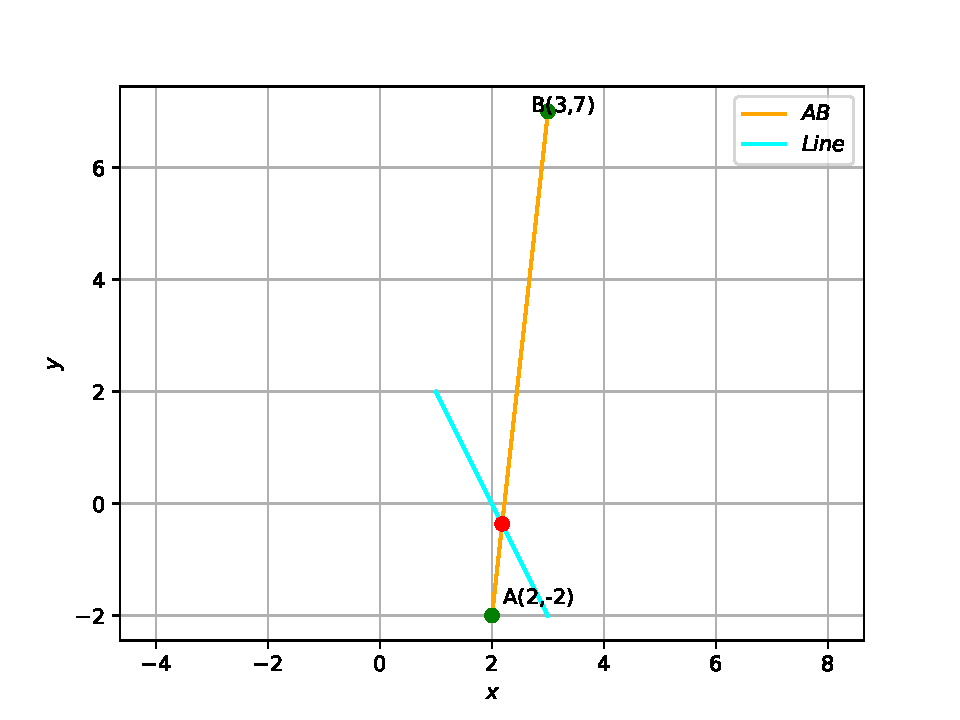
\includegraphics[width=\columnwidth]{/sdcard/IITH/vector/vector-1/figs/vec.pdf}
\caption{}
\label{fig:vec}
\end{figure}

\end{document}
